
\section{One word against two: the hard side}\label{sec:hard}

% gloss: One Word Against Two
This section proves part~(ii) of Theorem~\ref{thm:boundary}, the
PSPACE-hard half of Corollary~\ref{cor:algebraic},
Corollary~\ref{cor:real-complexity} on real path components and
Theorem~\ref{thm:rational-roots}.
In the shared-probe hardness reductions, exactly one word test compares one
word with two distinct words, and all other word tests compare single
words. With the specified probability floor and load-label calibrations,
the widened test forces a fixed positive sum at every probe. In the
constraint-logic reduction, each edge has its own probe, and either nonzero
summand makes its labeled end available as the tail.

% ---------------------------------------------------------------------------
\subsection{The load test}\label{sec:engine}

For the \defterm{load label}~$\mathsf u$ and labels $\mathsf x,\mathsf y$ we write $u_i$, $x_i$ and $y_i$
for their eigenvalues at probe~$i$.

% Lean: SingleAdditiveLicence.joint_words_iff (the 1+|I| equations), and
% the rate forcing in nclInstrument's legality proof.
\begin{lemma}[The load test]\label{lem:engine}
Let a shared-probe model have distinct labels $\mathsf u,\mathsf x,\mathsf
y$ among its $|M|$ labels, with probability floor $\delta=1/(|M|+1)$, and
let $k>0$ be rational. A parameter vector passes the word test
$\mathsf{uu}\sim\{\mathsf{xu},\mathsf{yu}\}$ and the calibrations
$u_i=k/2$ $(i\in I)$ if and only if $\theta_{\mathsf u}=2\delta$,
$\theta_m=\delta$ for every other label~$m$, $u_i=k/2$ and
\begin{equation}\label{eq:load}
  x_i+y_i=k\qquad\text{for every }i\in I.
\end{equation}
\end{lemma}

\begin{proof}
By Lemma~\ref{lem:compile}(b) the test says
$\theta_{\mathsf u}^2=(\theta_{\mathsf x}+\theta_{\mathsf y})\theta_{\mathsf u}$
and $\theta_{\mathsf u}^2u_i^2=\theta_{\mathsf u}(\theta_{\mathsf
x}x_i+\theta_{\mathsf y}y_i)u_i$ for $i\in I$. Since
$\theta_{\mathsf u}\ge\delta>0$, the first gives
$\theta_{\mathsf u}=\theta_{\mathsf x}+\theta_{\mathsf y}\ge2\delta$. The
other $|M|-1$ label probabilities are at least~$\delta$, and these lower
bounds sum to $(|M|+1)\delta=1$, so normalization forces equality
throughout. With $u_i=k/2>0$, the probe equations become
$\delta^2k^2=\delta^2k(x_i+y_i)$. The converse is the same computation.
\end{proof}

% gloss: load equation
In other words, with the label probabilities forced, each of the $|I|$
probe equations of the test becomes the \defterm{load equation}
\eqref{eq:load}, an affine trinomial in the eigenvalues. Since $k>0$, the
two summands never vanish together: a zero summand forces the other to
equal~$k$, although both may be nonzero in between
(Figure~\ref{fig:mechanism}(b)). %
In Figure~\ref{fig:mechanism}(a), setting $x=0$ makes both monomials
vanish, so $xy=xz$ ceases to constrain~$y$. By contrast, the held, calibrated load
equation $x_i+y_i=k>0$ retains its constraint when either summand
vanishes. Further tests decide which points of each load line are feasible,
and the number of probes grows with the input.

% ---------------------------------------------------------------------------
\subsection{The construction}\label{sec:construction}

% gloss: NCL
We reduce from nondeterministic constraint logic
(NCL)~\cite{hearndemaine}. An AND/OR constraint graph is a finite
multigraph $(V,E)$ whose edges have weights $\wt(e)\in\{1,2\}$ and labeled
ends $v_e^0,v_e^1$; each vertex meets incident weights $2,1,1$ (AND) or
$2,2,2$ (OR). Let $W(v)$ sum the weights over the ends at~$v$, so a loop
counts twice. An orientation $\sigma:E\to\{0,1\}$ makes $v_e^{\sigma(e)}$
the tail of $e$ and the other end its head. The orientation is legal if the heads at
every vertex carry weight at least two (minimum inflow two). Equivalently, since each end is a head or a
tail, the tails at every vertex~$v$ carry weight at most $W(v)-2$. A
flip reverses one edge between legal orientations. Hearn and
Demaine~\cite[Section~2 and Corollary~6]{hearndemaine} prove that deciding
whether flips lead from one supplied legal orientation to another is
PSPACE-hard, and their reduction produces distinct endpoints.

\begin{figure}[tbp]
  \centering
  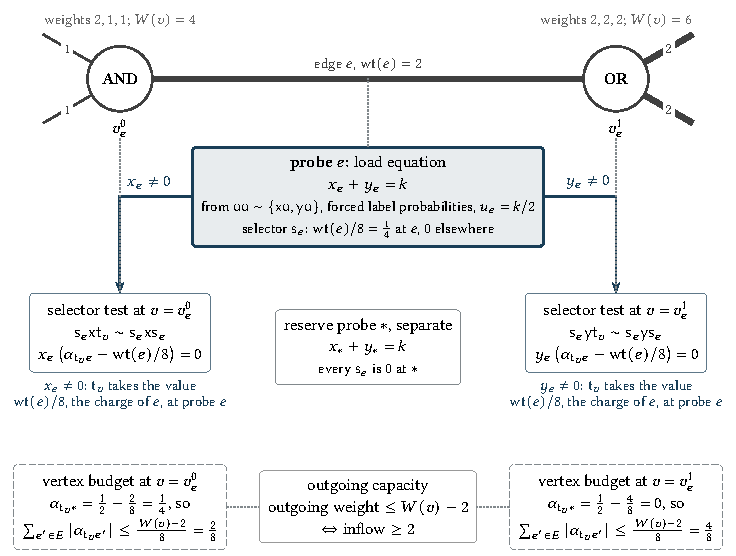
\includegraphics{figures/fig3-ncl-gadget.pdf}
  \Description{A gadget diagram. An AND vertex v_e^0 with edge weights 2, 1, 1 and an OR vertex v_e^1 with edge weights 2, 2, 2 are joined by the edge e of weight 2. The central box shows the load equation x_e + y_e = k at probe e, obtained from the word-against-pair test, the forced label probabilities and the calibration u_e = k/2. The selector s_e has eigenvalue wt(e)/8 = 1/4 at probe e and zero elsewhere. The arrow labelled x_e nonzero leads to the selector equation x_e (alpha_{t_{v_e^0}, e} - wt(e)/8) = 0 at the AND vertex. The arrow labelled y_e nonzero leads to y_e (alpha_{t_{v_e^1}, e} - wt(e)/8) = 0 at the OR vertex. The reserve probe has its own load equation, and every selector has eigenvalue zero there. The dashed boxes show reserve calibrations 1/4 at the AND vertex and 0 at the OR vertex, leaving edge-probe budgets 2/8 and 4/8, respectively. On a canonical orientation lift, each budget is equivalent to outgoing weight at most W(v) - 2, hence to inflow at least 2.}
  \caption{One NCL edge becomes one probe, on which the two summand eigenvalues share the load~$k$. A nonzero summand requires the vertex label at that end of the edge to take the value $\wt(e)/8$, the \emph{charge} of~$e$, at probe~$e$.
% gloss: charge
On a canonical orientation lift, the vertex budget is equivalent to NCL's minimum inflow of two; for an arbitrary feasible configuration, every orientation obtained by choosing one nonzero summand at each edge satisfies minimum inflow two at every vertex. Here the edge~$e$, of weight two, joins an AND vertex $v_e^0$ (edge weights $2,1,1$) to an OR vertex $v_e^1$ (edge weights $2,2,2$); an edge between an AND vertex and an OR vertex always has weight two. The selector $\mathsf s_e$ has eigenvalue $\wt(e)/8$ at probe~$e$ and $0$ at every other probe. The forced label probabilities give the two words of each selector test equal word probabilities, so after cancelling $\wt(e)/8$ the tests $\mathsf s_e\mathsf x\mathsf t_{v_e^0}\sim\mathsf s_e\mathsf x\mathsf s_e$ and $\mathsf s_e\mathsf y\mathsf t_{v_e^1}\sim\mathsf s_e\mathsf y\mathsf s_e$ give the selector equations shown.
% gloss: selector equations
The calibration of $\mathsf t_v$ at the reserve probe~$\ast$ leaves the budget $\sum_{e'\in E}|\alpha_{\mathsf t_ve'}|\le(W(v)-2)/8$, which is $1/4$ at the AND vertex and $1/2$ at the OR vertex. The reserve probe carries its own load equation and no selector. Together with the forced label probabilities, the calibrations and the remaining model constraints, including all per-label budgets, the displayed equations characterize the feasible configurations.}\label{fig:ncl}
\end{figure}

% gloss: reserve probe
% gloss: load label
% gloss: summand labels
% gloss: selector labels
% gloss: vertex labels
Given a graph and legal orientations $\sigma,\tau$, the reduction outputs
the following model. The probes are $I=E\sqcup\{\ast\}$, one per edge and a
\defterm{reserve probe}~$\ast$ for the unused part of each vertex
budget~\eqref{eq:vertex-budget}. The base is $X=\mathbb F_2^d$ with
$d=\lceil\log_2(|E|+2)\rceil$, and
$\chi_i(g)=(-1)^{a_i\cdot g}$ for distinct nonzero $a_i\in X$. The labels,
each its own reversal, are the load label~$\mathsf u$; the
\defterm{summand labels} $\mathsf x,\mathsf y$, which choose tails;
\defterm{selector labels} $\mathsf s_e$ $(e\in E)$, which read the summands
at probe~$e$; and \defterm{vertex labels} $\mathsf t_v$ $(v\in V)$. So
$|M|=|E|+|V|+3$, and we put
\[
  \delta=\frac1{|M|+1},\qquad k=\frac1{4|I|},\qquad\kappa=\frac12,\qquad
  H=3,
\]
with a one-value register and only level~$0$. The value tests are the
calibrations
\[
  u_i=\frac k2\ \ (i\in I),\qquad
  \alpha_{\mathsf s_ei}=
  \begin{cases}\wt(e)/8,&i=e,\\0,&i\neq e,\end{cases}\qquad
  \alpha_{\mathsf t_v\ast}=\frac12-\frac{W(v)-2}8 .
\]
The word tests are the load test and two \defterm{selector tests} per
edge:
\[
  \mathsf{uu}\sim\{\mathsf{xu},\mathsf{yu}\},\qquad
  \mathsf s_e\mathsf x\mathsf t_{v_e^0}\sim\mathsf s_e\mathsf x\mathsf s_e,
  \qquad
  \mathsf s_e\mathsf y\mathsf t_{v_e^1}\sim\mathsf s_e\mathsf y\mathsf s_e .
\]
The only admissible set is the full word-test list. The profile $p$ has
full table support and holds every test.

% gloss: charge
% gloss: selector equations
% gloss: vertex budgets
We call $\wt(e)/8$ the \defterm{charge} of~$e$; the vertex budgets below
cap the tails' total charge at each vertex, as legality caps their weight. The selector tests give the
\defterm{selector equations}~\eqref{eq:selector} below: the vertex label at
an end of~$e$ takes the charge at probe~$e$ whenever that end's summand is
nonzero (Figure~\ref{fig:ncl}). The \defterm{canonical orientation lift} $A_\sigma$ of
$\sigma$ has label probabilities $2\delta$ at $\mathsf u$ and $\delta$
elsewhere, the calibrated eigenvalues, $(x_\ast,y_\ast)=(k,0)$, and
$(x_e,y_e)$ equal to $(k,0)$ or $(0,k)$ as $\sigma(e)$ is $0$ or~$1$. Its
label $\mathsf t_v$ takes the charge of~$e$ at probe~$e$ if $v$ is the
tail of~$e$, and $0$ otherwise. The reduction outputs the model, $p$,
$A_\sigma$, $A_\tau$ and, for the supplied-tolerance variant,
$\varepsilon_0=\delta k/(2|X|+1)$; it runs in polynomial time
(Appendix~\ref{app:ncl-size}).

% ---------------------------------------------------------------------------
\subsection{Feasible configurations}\label{sec:feasible}

The next lemma lists exactly what feasibility at~$p$ requires.

\begin{lemma}[Feasible configurations]\label{lem:feasible}
In the construction of Section~\ref{sec:construction}, a rational parameter
vector gives a feasible configuration at~$p$ if and only if it satisfies
the conditions below and the remaining model constraints. These include
the calibrations and the $\ell^1$ budget of every label. The conditions
are $\theta_{\mathsf u}=2\delta$ and $\theta_m=\delta$ for $m\neq\mathsf
u$, the load equation~\eqref{eq:load} at every probe, the selector
equations
\begin{equation}\label{eq:selector}
  x_e\Bigl(\alpha_{\mathsf t_{v_e^0}e}-\frac{\wt(e)}8\Bigr)=0,\qquad
  y_e\Bigl(\alpha_{\mathsf t_{v_e^1}e}-\frac{\wt(e)}8\Bigr)=0\qquad(e\in E)
\end{equation}
% gloss: vertex budgets
and the \defterm{vertex budgets}
\begin{equation}\label{eq:vertex-budget}
  \sum_{e\in E}|\alpha_{\mathsf t_ve}|\le\frac{W(v)-2}8\qquad(v\in V).
\end{equation}
\end{lemma}

\begin{proof}
The register, support, reversal and admissibility conditions hold here by
construction, so feasibility means Definition~\ref{def:model} and every
held test. Lemma~\ref{lem:engine} handles the load test and the
calibrations of~$\mathsf u$. In a selector test both words have three
labels of probability~$\delta$, and at probe~$i$
Lemma~\ref{lem:compile}(a) requires
$\alpha_{\mathsf s_ei}x_i\alpha_{\mathsf t_{v_e^0}i}=\alpha_{\mathsf
s_ei}^2x_i$. Both sides vanish for $i\neq e$; at $i=e$, cancelling
$\wt(e)/8>0$ gives~\eqref{eq:selector}, and likewise with~$\mathsf y$.
Since $\alpha_{\mathsf t_v\ast}\ge0$, the budget of $\mathsf t_v$
is~\eqref{eq:vertex-budget}.
\end{proof}

The listed equations alone do not suffice: the reserve pair
$(x_\ast,y_\ast)=(1,k-1)$ satisfies all of them but violates the budget
of~$\mathsf x$.

% gloss: available
% gloss: represented
To read orientations off a feasible configuration at~$p$, call the end
$v_e^0$ of $e$ \defterm{available} if $x_e\neq0$, and $v_e^1$ if $y_e\neq0$. An
orientation is \defterm{represented} if the tail of every edge is
available. By~\eqref{eq:load} every edge has an available end, and since
both summands may be nonzero, a feasible configuration can represent
several orientations. On a canonical orientation lift, the vertex budget is
equivalent to minimum inflow two. At any feasible configuration, each
represented outgoing edge forces its full charge in a distinct probe
coordinate at its chosen vertex, so every mixture of represented choices is
legal. Hence two orientations represented by one configuration are joined
by legal flips through orientations it represents. The lift $A_\sigma$
represents only~$\sigma$, so distinct orientations give distinct feasible
endpoints (Appendix~\ref{app:ncl-transfer}).

% ---------------------------------------------------------------------------
\subsection{Both directions of the transfer}\label{sec:transfer}

Fix an instance of the construction. It remains to decode sequences into
legal flips and to lift flips to sequences. Decoding must handle every
feasible step below~$\varepsilon_0$, including
steps that change many coordinates or pass through negative summands, and
configurations representing several orientations.

% Lean: ConstraintLogic common_orientation, flips_of_represents,
% legal_of_represents.
\begin{lemma}[Small steps share an orientation]\label{lem:decode}
Let $A$ and $B$ be feasible configurations at~$p$ whose summands satisfy
$|x_{A,e}-x_{B,e}|<k$ for every $e\in E$. Then some orientation is
represented by both. Hence, if consecutive configurations of a
reconfiguration sequence from $A_\sigma$ to $A_\tau$ satisfy this bound,
legal flips lead from $\sigma$ to~$\tau$.
\end{lemma}

% Lean: Graph.flip_segments_lawful; the encoder clips the summands to
% [0,k], which is the identity on the three segments.
\begin{lemma}[Legal flips lift]\label{lem:lift}
If $\tau$ arises from a legal orientation $\sigma$ by one legal flip, then
for every rational $\varepsilon>0$ a reconfiguration sequence at
tolerance~$\varepsilon$ leads from $A_\sigma$ to~$A_\tau$.
\end{lemma}

% Lean: ncl_chain_iff (at the supplied cutoff) and ncl_fine_iff (fine
% reachability); the smaller-tolerance case combines them with
% monotonicity in writing.
\begin{lemma}[The cutoff]\label{lem:cutoff}
Let $\sigma,\tau$ be legal orientations. For every rational $0<\varepsilon\le\varepsilon_0$ the
following are equivalent: legal flips lead from $\sigma$ to~$\tau$;
$A_\tau$ is finely reachable from~$A_\sigma$; a reconfiguration sequence at
tolerance $\varepsilon$ leads from $A_\sigma$ to~$A_\tau$.
\end{lemma}

\begin{proof}[Proof idea for Lemmas~\ref{lem:decode}--\ref{lem:cutoff}]
At an edge, disjoint available ends at $A$ and $B$ would make $x_e$ jump
between $0$ and~$k$, by~\eqref{eq:load}. Choosing a common available end at
each edge gives a common represented orientation, whatever the signs.
At the forced label probabilities, summing a row for label~$m$ with
weights $\chi_i(g)\chi_i(h)$ gives $\theta_m\alpha_{mi}$. A step below
$\varepsilon_0$ therefore changes each eigenvalue by less than
$|X|\varepsilon_0/\delta<k$, so adjacent configurations share an available
end at every edge. To lift a flip with distinct tails, preload the new tail, interpolate
the summands, and unload the old tail. Each preloaded vertex total is the
larger of its two endpoint totals. For a loop, keep its one charge fixed
and interpolate only the summands. For the cutoff, any sequence at $0<\varepsilon\le\varepsilon_0$ is also one at
$\varepsilon_0$ and decodes to legal flips. Conversely, legal flips lift to
sequences at every positive tolerance.
Appendix~\ref{app:ncl-transfer} gives the full argument.
\end{proof}

As noted after Theorem~\ref{thm:boundary}, this agreement can fail at
larger tolerances.

% ---------------------------------------------------------------------------
\subsection{Length one, and the proof of Theorem~\ref{thm:boundary}(ii)}\label{sec:length-one}

% Lean: the `short` parameter of nclInstrument and of every ncl_* theorem
% gives each length separately; the cancellation is written.
\begin{proposition}[A word-against-pair test of length one]\label{prop:length-one}
Replace $\mathsf{uu}\sim\{\mathsf{xu},\mathsf{yu}\}$ by
$\mathsf u\sim\{\mathsf x,\mathsf y\}$ in the construction, keeping every
other input, including the held load calibrations, $H=3$ and both
endpoints. Then the feasible
configurations at~$p$, and hence the reconfiguration sequences at every
tolerance, are unchanged.
\end{proposition}

\begin{proof}
By Lemma~\ref{lem:compile}(b), the mass equation of the length-two test is
$\theta_{\mathsf u}$ times that of the length-one test, and its equation at
probe~$i$ is $\theta_{\mathsf u}u_i$ times the corresponding length-one
equation. The probability floor gives $\theta_{\mathsf u}>0$, and the calibration gives
$u_i=k/2>0$ at every probe, the reserve included.
\end{proof}

This reduction works with the unique word-against-pair test of length one
or two.

\begin{proof}[Proof of Theorem~\ref{thm:boundary}(ii)]
Map an NCL instance $(V,E,\sigma,\tau)$ to the construction of
Section~\ref{sec:construction}, using the word-against-pair test of length
two (or one, by Proposition~\ref{prop:length-one}). The map runs in
polynomial time, and its endpoints are feasible at~$p$. By
Lemma~\ref{lem:cutoff}, legal flips lead from $\sigma$ to $\tau$ exactly
when $A_\tau$ is finely reachable from $A_\sigma$, and exactly when a
sequence exists at the supplied tolerance $\varepsilon_0$. Here
$1/\varepsilon_0=(|M|+1)\cdot4|I|\cdot(2|X|+1)$ is polynomially bounded.
The instances have the restrictions listed in Theorem~\ref{thm:boundary},
and distinct orientations give distinct endpoints. By Remark~\ref{rem:inputs}(ii) the bounds also hold
with profile steps allowed, which gives the last claim of
Theorem~\ref{thm:directed}.
\end{proof}

Thus PSPACE-hardness needs only one word-against-pair test, at one
profile, so it comes from neither profile steps nor the order in which
tests are acquired. The next remark replaces that one test.

\begin{remark}[One word test crosses the boundary]\label{rem:control}
Replace the length-two word-against-pair test by
$\mathsf{uu}\sim\mathsf{uu}$ in the same place in the word-test list, with
every other input fixed. This preserves the supplied feasible endpoints and their common profile,
and puts the instance in the single-word class. The three-segment witness
(damp the summand eigenvalues at the original label probabilities,
interpolate the vertex-label eigenvalues inside their budgets, undamp at
the target) gives a yes verdict at every positive tolerance. For
disconnected NCL endpoints the verdict changes from no
(Lemma~\ref{lem:cutoff}) to yes. In $K_{3,3}$ with a weight-two perfect
matching and weight one elsewhere, every vertex is an AND vertex. Orienting
the matching toward one side and the other edges toward the other side, or
the reverse, gives such a pair: every vertex has inflow exactly two, so no
flip is legal.
\end{remark}

At the end of the first segment after replacement, both summands vanish at
every probe, which the original load equation forbids. For the disconnected
endpoint pair above, replacing that one test changes the verdict from no
to yes with every other input fixed (Appendix~\ref{app:ncl-control}). This change is not evidence that the test's shape
alone causes hardness. In part~(ii), other word tests and calibrations are
unrestricted in number, and we claim no necessity for the probability
floor, calibrations, budgets, selectors, reserve or growing probe family.

\subsection{The algebraic form, second half, and real path components}\label{sec:real-ncl}

The same mechanism, without the Markov model, gives the PSPACE-hard half
of Corollary~\ref{cor:algebraic}. The direct algebraic reduction discards
the reserve and uses one normalized affine trinomial per edge; dividing every load
equation of Section~\ref{sec:construction} by $k$ would also retain the
reserve equation. For a
constraint graph with legal orientations $\sigma,\tau$, take coordinates
$x_{e0},x_{e1}$ $(e\in E)$ and $z_{ve}$ $(v\in V,\ e\in E)$ with
\begin{equation}\label{eq:ncl-system}
  x_{e0}+x_{e1}=1,\qquad
  x_{eb}\,z_{v_e^be}=\wt(e)\,x_{eb},\qquad
  |x_{eb}|\le1,\qquad
  \sum_{e\in E}|z_{ve}|\le W(v)-2.
\end{equation}
The endpoint of $\sigma$ has $x_{e\sigma(e)}=1$, $x_{e,1-\sigma(e)}=0$, and
$z_{ve}=\wt(e)$ if $v$ is the selected tail of~$e$, and $z_{ve}=0$
otherwise. Feasible configurations of Section~\ref{sec:construction} map
into this system by dividing the summands by~$k$, clipping them to $[0,1]$, and
dividing the vertex-label eigenvalues by $1/8$. The budgets bound every coordinate.
Lemmas~\ref{lem:decode} and~\ref{lem:lift} apply with unit
summands and sup-norm steps strictly below~$1$ for decoding; the lift gives
sequences at every positive tolerance. So the endpoints are finely
connected exactly when legal flips lead from $\sigma$ to~$\tau$
(Appendix~\ref{app:ncl-algebraic}). There are $|E|$ normalized affine
trinomials, so their number grows. Theorem~\ref{thm:boundary}(ii) counts
exactly one word-against-pair test.

Nor does part~(ii) give hardness with one scalar equation. After
calibration and forcing of the label probabilities, the loads are affine
equations, one per probe. Selector equations link each edge's summands to
the vertex labels' eigenvalues at that probe, and per-label budgets couple
coordinates across probes. The paper leaves PSPACE-hardness with one
scalar affine trinomial open.

The same instances give the PSPACE-hardness in
Corollary~\ref{cor:real-complexity}. The three segments of
Lemma~\ref{lem:lift}, in the coordinates~\eqref{eq:ncl-system}, lift legal
flips to piecewise-linear real paths. Conversely, sample a real path
between the endpoints with consecutive samples at sup distance strictly
below one; as in Lemma~\ref{lem:decode}, adjacent samples represent a
common orientation, which gives legal flips from $\sigma$ to~$\tau$
(Appendix~\ref{app:ncl-algebraic}).

% gloss: P-complete
\begin{corollary}[Complexity of real path components]\label{cor:real-complexity}
Consider explicitly binary-encoded budgeted signed-binomial systems and two
supplied feasible rational endpoints. Deciding whether the endpoints lie in
the same path component of the full real feasible locus is P-complete under
deterministic log-space many-one reductions whose outputs satisfy the
feasibility promise.
% gloss: PSPACE-hard
If the language also allows an input-dependent number of scalar equations
$x_j+y_j=1$, this real decision problem is PSPACE-complete under
polynomial-time many-one reductions whose outputs satisfy the feasibility
promise. Neither upper bound needs a boundedness promise. PSPACE-hardness
already holds for bounded real feasible loci.
\end{corollary}

\begin{proof}
In the binomial-only language, Corollary~\ref{cor:real} identifies the
real verdict with equality of signed cores.
The algorithm of Section~\ref{sec:algorithm} computes both signed cores from the
endpoints and the test list, and none of its steps uses a bound on the
feasible set. The circuit transfer of Section~\ref{sec:circuit-transfer},
from monotone circuit value~\cite{goldschlager}, gives the P-hardness. The
real transfer of this section, from NCL~\cite{hearndemaine}, gives the
PSPACE-hardness. The PSPACE upper bound uses the component description of
Heintz, Roy and Solern\'o~\cite{heintzroysolerno1994components} after a
polynomial-time translation to degree two (Appendix~\ref{app:hrs}).
\end{proof}

Thus the hardness sources of Corollary~\ref{cor:real-complexity},
monotone circuit value and constraint logic, are imported, and the PSPACE upper bound uses the external component algorithm; the contribution is the complexity of this restricted
algebraic language. General semialgebraic roadmap algorithms decide the
real two-endpoint problem with trinomials~\cite{basupollackroy}. The
result gives no upper bound for rational fine connectivity with
trinomials (Corollary~\ref{cor:algebraic}), and no agreement between that
verdict and real path-component membership.

% ---------------------------------------------------------------------------
\subsection{Rational roots}\label{sec:rational-roots}

We prove no upper bound for part~(ii) of Theorem~\ref{thm:boundary}: one
word-against-pair test with probes already encodes the existence of
rational zeros, Hilbert's tenth problem over~$\QQ$.
% gloss: Hilbert's tenth problem over Q

Let $f$ be an integer polynomial, sparsely encoded in binary with
length~$\mathcal L$. Binary doubling and repeated squaring give a straight-line
program with $O(\mathcal L+1)$ gates~$\gamma$ whose last gate computes~$f$, as in the
substitutions behind Shor normal form~\cite[Section~3.3, proof of Theorem~1(3)]{bihanrojasstella}.
Its gates are inputs, constants $0$ and~$1$, sums, negations and products.
Work in the box $z_\gamma\in[-1,1]$, $\zeta\in[0,2]$, $\xi\in[1,3]$,
$\psi\in[-1,1]$ and $s\in[0,2]$, with $s$ the \defterm{switch}. Homogenize every gate equation with~$\zeta$ (a product
reads $\zeta z_\gamma=z_{\gamma'}z_{\gamma''}$), require $z_\gamma=0$ at
the last gate, add $\xi^2=2+\zeta^2\psi$, and multiply every residual by
the switch factor $s(2-s)$. The endpoints at $s=0$ and $s=2$ are
therefore feasible whatever $f$ is. At a rational point with $0<s<2$,
$\zeta=0$ would give $\xi^2=2$, so $\zeta>0$ and the inputs of
$z_\gamma/\zeta$ form a rational root.

Normalize to coordinates $t_j\in[0,1]$. Products become squares through
$2tt'=4\bar t^2-t^2-t'^2$ with $\bar t=(t+t')/2$, and each affine equality
and square becomes two inequalities
$\sum_jc_{\rho j}|t_j^{a_j}(1-t_j)^{b_j}|\le c_\rho$ with $c_{\rho j}\ge0$
and $a_j+b_j\le2$. The model compiles these inequalities using the length-one load test, a
reserve probe, and one probe per coordinate or copy. Copies serve repeated
occurrences. At each coordinate or copy probe~$j$, read $t_j=x_j/k$. The
model uses calibrated probe-selector labels~$\mathsf o_j$, a calibrated
pad label~$\mathsf p$ matching word lengths, calibrated coefficient
labels~$\mathsf c_{\rho j}$, and an inequality label~$\mathsf r_\rho$ for
each~$\rho$. For each inequality~$\rho$, the single-word tests
\[
  \mathsf o_j\mathsf r_\rho\mathsf p^{a_j+b_j}\sim
  \mathsf o_j\mathsf c_{\rho j}\mathsf x^{a_j}\mathsf y^{b_j}
\]
force $\alpha_{\mathsf r_\rho j}$ to be a fixed positive multiple of
$c_{\rho j}t_j^{a_j}(1-t_j)^{b_j}$. The reserve calibration of
$\mathsf r_\rho$ then turns its $\ell^1$ budget into inequality~$\rho$.

% Lean: ResponseBudgets.assign_lawful, decode_solution, decode_lift,
% lift_chain, decode_chain, fine_iff_box, no_native_chain_of_selector
% (assumes the selector dichotomy; deriving it is written);
% CalibratedResponses.rates_eq, lawful_state, build_decode.
\begin{theorem}[Rational roots]\label{thm:rational-roots}
There is a polynomial-time many-one reduction from the existence of a
rational zero of a sparsely binary-encoded integer polynomial to Fine
Reachability at a fixed profile. Its shared-probe models have exactly one
word-against-pair test, of length one, other word tests of length at most
four, a one-value register, identity reversal, $\kappa=1/2$ and a growing
number of probes. Both endpoints are feasible at one profile holding every
test. The same reduction works for sequence
existence at the supplied tolerance $\varepsilon_0=\delta k/(2|X|+1)$ and
at every smaller positive tolerance.
\end{theorem}

\begin{proof}[Proof idea]
If $f$ has a rational root, two segments in the end faces and one
intervening switch segment lift by polynomial maps. These maps are
uniformly continuous on the box, so rational subdivision gives sequences at
every positive tolerance. If $f$ has no rational root, every feasible
configuration at the common profile has $t_s\in\{0,1\}$. A switch between
these values changes the corresponding eigenvalue by~$k$, which is
impossible at any $0<\varepsilon\le\varepsilon_0$. Appendix~\ref{app:rational-roots} gives
the compiler and its bounds.
\end{proof}

So a PSPACE upper bound for part~(ii) would put the existence of rational
zeros of integer polynomials in PSPACE.
% gloss: undecidable
A 2026 preprint~\cite{openaih10q}, reported by Sun~\cite[Section~1]{sun},
claims that Hilbert's tenth problem over~$\QQ$ is undecidable; if that
claim holds, so is the problem of part~(ii). We use the reported claim only
conditionally and have not checked its arithmetic proof. The reduction is
independent of the claim.

The usual finite-graph PSPACE argument would require a polynomial encoding
bound for the vertices needed in the search.
Proposition~\ref{prop:long-sequences} shows that explicit rational sequences
in the algebraic problem can require points of superpolynomial binary
length even at a fixed tolerance. Fine reachability also quantifies over
every positive tolerance. These issues arise already with symmetric
adjacency at a fixed profile.

% ---------------------------------------------------------------------------
\subsection{Fixed counts: the quartic layout}\label{sec:quartic}

For quartics in a fixed number of variables, a fixed \emph{layout} of labels, probes and tests keeps every
count of Theorem~\ref{thm:rational-roots} fixed. The counts and lengths of
the words are fixed; the word records themselves can depend on the signs
of the coefficients.

% Lean: QuarticSelector.homogeneous_scale, interior_hasRoot,
% no_root_selector, root_has_three_segments; RowRealization.native_boundary
% and RowRealization.nativeEndpoints_distinct take a RowRealization as
% input (lift, readback and slope proofs). Row assembly, bit bounds and the
% conditional transfer are written.
\begin{corollary}[Fixed counts]\label{cor:quartic}
Fix $N$. There is a polynomial-time many-one reduction from rational
solvability of integer polynomials of total degree at most four
in $N$ variables to (a)~Fine Reachability at a fixed profile and
(b)~sequence existence at one prescribed positive rational tolerance. The
targets are shared-probe models with exactly one word-against-pair test, of
length one, and other word tests of length at most four. They have a
one-value register, identity reversal, $\kappa=1/2$ and the full word-test
list as the only admissible set. Both endpoints have one full-support profile with
only level~$0$ and every test held. The numbers of probes, labels, base
states, word tests and value tests, and the tolerance in~(b), depend only
on~$N$. If
the Bhargava--Burungale quartic theorem~\cite[Corollary~1.2(3)]{bhargavaburungale} holds, both problems are undecidable for
some fixed numbers of probes and labels, problem~(b) at the corresponding
fixed tolerance.
\end{corollary}

\begin{proof}[Proof idea]
Use the dense homogenization
$F(z,\zeta)=\sum_{|a|\le4}c_az^a\zeta^{4-|a|}$ with the switch
$s\in[0,1]$ and the equations $s(1-s)F(z,\zeta)=0$ and
$s(1-s)(\xi^2-2-\zeta^2\psi)=0$; then $F(\zeta v,\zeta)=\zeta^4f(v)$.
Compute the monomial slots of degrees one to six in the $N+4$ normalized
coordinates by a fixed sequence of products, and compile as in
Theorem~\ref{thm:rational-roots}. The unique
word-against-pair test has length one. All other word tests have length at
most four, including the degree-two square slots. Both supplied endpoints
lift: each corner satisfies the gated residuals, and the polynomial
assignment satisfies every gadget constraint, including those of the
product $s\cdot s$ at $s=1$. The cutoff $\varepsilon_0$ depends only on the layout, and each
calibration has binary length $O_N(\mathcal L+1)$ for input length~$\mathcal L$
(Appendix~\ref{app:quartic}).
\end{proof}

The Bhargava--Burungale quartic theorem, Corollary~1.2(3) of their
preprint, states that rational
solvability of integer quartics in some fixed number of variables is
undecidable. It is in a preprint (arXiv 2611.16130v2) with no refereed
version identified, and we use only its statement. Fixed counts and a fixed
cutoff still allow input-dependent rational calibration values. The
reduction settles neither the case of no probes nor the least sufficient
number of probes.
